The NavIC transmitter is simulated to send baseband signal to the channel as shown in Fig \ref{fig:trans_flow}. 

\begin{figure}[ht]
\centering
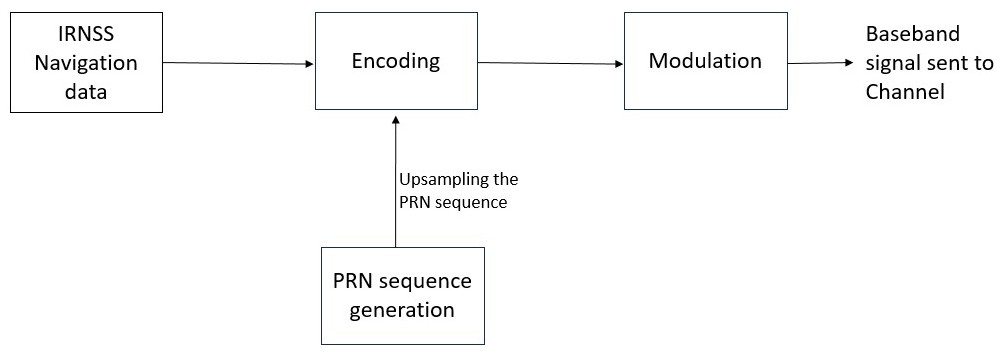
\includegraphics[width=1\columnwidth]{figs/trans_flow.jpg}
\centering
\captionsetup{justification=centering}
\caption{Transmitter Block diagram}
\label{fig:trans_flow}
\end{figure}

\section{IRNSS Navigation data}
Navigation data in satellite communication refers to the crucial information transmitted between satellites and ground-based receivers to facilitate accurate positioning and navigation. It includes data related to satellite orbits, precise timing, and other parameters necessary for determining the satellite's position relative to the Earth's surface.
\section{Frame structure}
NavIC master frame consists of $2400$ symbols, divided into $4$ subframes. Each subframe is $600$ symbols long. Each subframe has $16$ bit Sync word followed by $584$ bits of interleaved data. Subframes $1$ and $2$ transmit fixed primary navigation parameters. Subframe $3$ and $4$ transmit secondary navigation parameters in the form of messages. The master frame structure is shown in figure \ref{fig:master_frame}. 

\begin{figure}[ht]
\centering
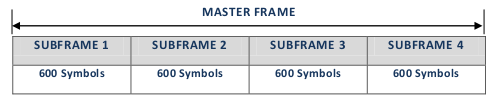
\includegraphics[width=0.8\columnwidth]{figs/master_frame.png}
\centering
\captionsetup{justification=centering}
\caption{Master Frame Structure}
\label{fig:master_frame}
\end{figure}

\noindent Each subframe is $292$ bits long without FEC encoding and sync word. It starts with TLM word of 8 bits and ends with $24$ bit Cyclic Redundancy Check(CRC) followed by $6$ tail bits. In subframes $1$ and $2$ navigation data is alloted with $232$ bits, starting from bit $31$. In subframe $3$ and $4$, $220$ bits are alloted starting from bit $37$. The typical structure of the subframes are shown in figure \ref{fig:frame_1_2} and figure \ref{fig:frame_3_4} respectively.

\begin{figure}[ht]
\centering
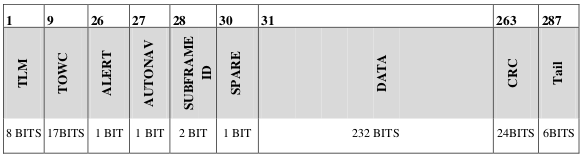
\includegraphics[width=0.8\columnwidth]{figs/1_2.png}
\centering
\captionsetup{justification=centering}
\caption{Structure of subframe 1 and 2}
\label{fig:frame_1_2}
\end{figure}

\begin{figure}[ht]
\centering
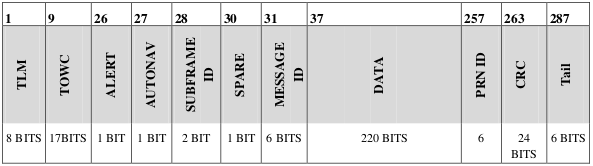
\includegraphics[width=0.8\columnwidth]{figs/3_4.png}
\centering
\captionsetup{justification=centering}
\caption{Structure of subframe 3 and 4}
\label{fig:frame_3_4}
\end{figure}

\section{Moduation and Encoding}
\subsection{PRN codes for SPS}
Direct Sequence Spread Spectrum (DSSS), an extension of BPSK modulation, is utilized in NavIC signal modulation. We multiply the signal with a Pseudo Random waveform, thereby increasing the bandwidth occupied. PRN Codes selected for Standard Positioning System are similar to GPS C/A Gold codes. The length of each code is $1023$ chips. The code is chipped at $1.023$ Mcps.

\noindent For SPS code generation, the two polynomials G1 and G2 are as defined below:
\begin{align}
G1 &: X^{10}+X^{3} + 1\\
G2 &: X^{10}+X^9+X^8+X^6+X^3+X^2+1
\end{align}
Polynomial G1 and G2 are similar to the ones used by GPS C/A signal. The G1 and G2 generators are realized by using $10$ bits Maximum Length Feedback Shift Registers(MLFSR). The initial state of G2 provides the chip delay. The G1 register is initialized with all bits as $1$. G1 and G2 are XOR'ed for the generation of the final $1023$ chip long PRN sequence. The SPS PRN code generator is shown in figure \ref{figure:codeGen}.

\begin{figure}[!ht]
	\centering
	\tikzset{every picture/.style={line width=0.75pt}} %set default line width to 0.75pt        

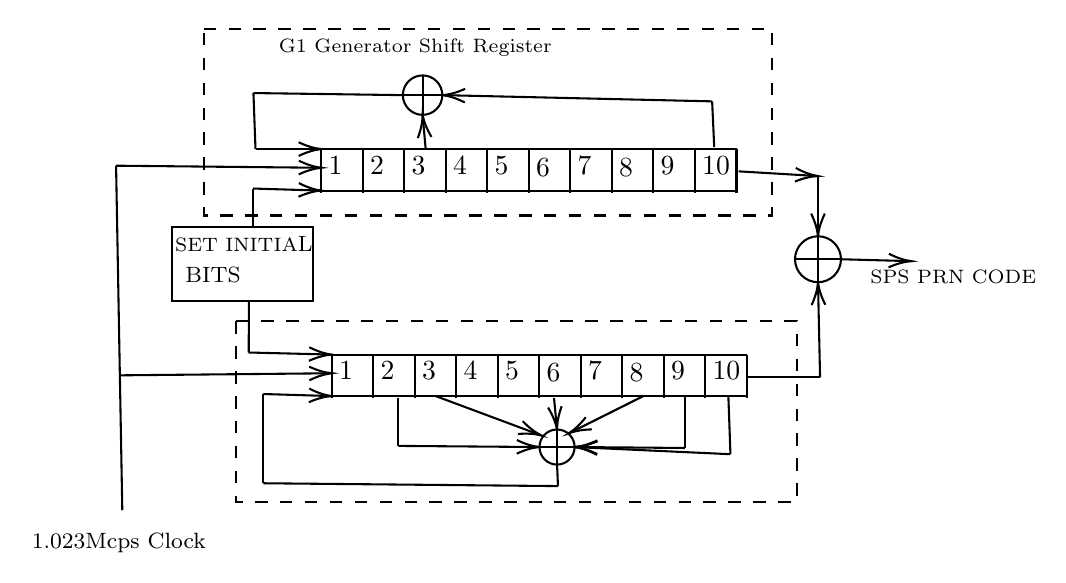
\begin{tikzpicture}[x=0.75pt,y=0.75pt,yscale=-1,xscale=1]
%uncomment if require: \path (0,300); %set diagram left start at 0, and has height of 300

%Shape: Grid [id:dp4759069175630535] 
\draw  [draw opacity=0] (187,78.28) -- (387.09,78.28) -- (387.09,99.28) -- (187,99.28) -- cycle ; \draw   (187,78.28) -- (187,99.28)(207,78.28) -- (207,99.28)(227,78.28) -- (227,99.28)(247,78.28) -- (247,99.28)(267,78.28) -- (267,99.28)(287,78.28) -- (287,99.28)(307,78.28) -- (307,99.28)(327,78.28) -- (327,99.28)(347,78.28) -- (347,99.28)(367,78.28) -- (367,99.28)(387,78.28) -- (387,99.28) ; \draw   (187,78.28) -- (387.09,78.28)(187,98.28) -- (387.09,98.28) ; \draw    ;
%Straight Lines [id:da569456764054443] 
\draw    (88.09,86.28) -- (185.09,87.26) ;
\draw [shift={(187.09,87.28)}, rotate = 180.58] [color={rgb, 255:red, 0; green, 0; blue, 0 }  ][line width=0.75]    (10.93,-3.29) .. controls (6.95,-1.4) and (3.31,-0.3) .. (0,0) .. controls (3.31,0.3) and (6.95,1.4) .. (10.93,3.29)   ;
%Straight Lines [id:da10333590103804569] 
\draw    (155.27,78.28) -- (185,78.28) ;
\draw [shift={(187,78.28)}, rotate = 180] [color={rgb, 255:red, 0; green, 0; blue, 0 }  ][line width=0.75]    (10.93,-3.29) .. controls (6.95,-1.4) and (3.31,-0.3) .. (0,0) .. controls (3.31,0.3) and (6.95,1.4) .. (10.93,3.29)   ;
%Straight Lines [id:da24492265686656967] 
\draw    (154.09,97.28) -- (185,98.22) ;
\draw [shift={(187,98.28)}, rotate = 181.74] [color={rgb, 255:red, 0; green, 0; blue, 0 }  ][line width=0.75]    (10.93,-3.29) .. controls (6.95,-1.4) and (3.31,-0.3) .. (0,0) .. controls (3.31,0.3) and (6.95,1.4) .. (10.93,3.29)   ;
%Straight Lines [id:da7870160753562048] 
\draw    (88.09,86.28) -- (91.09,252.28) ;
%Shape: Grid [id:dp16213094638707903] 
\draw  [draw opacity=0] (192,177.28) -- (392.09,177.28) -- (392.09,198.28) -- (192,198.28) -- cycle ; \draw   (192,177.28) -- (192,198.28)(212,177.28) -- (212,198.28)(232,177.28) -- (232,198.28)(252,177.28) -- (252,198.28)(272,177.28) -- (272,198.28)(292,177.28) -- (292,198.28)(312,177.28) -- (312,198.28)(332,177.28) -- (332,198.28)(352,177.28) -- (352,198.28)(372,177.28) -- (372,198.28)(392,177.28) -- (392,198.28) ; \draw   (192,177.28) -- (392.09,177.28)(192,197.28) -- (392.09,197.28) ; \draw    ;
%Straight Lines [id:da7354388024747429] 
\draw    (90.09,187.28) -- (190.09,186.3) ;
\draw [shift={(192.09,186.28)}, rotate = 179.44] [color={rgb, 255:red, 0; green, 0; blue, 0 }  ][line width=0.75]    (10.93,-3.29) .. controls (6.95,-1.4) and (3.31,-0.3) .. (0,0) .. controls (3.31,0.3) and (6.95,1.4) .. (10.93,3.29)   ;
%Straight Lines [id:da7447494470460669] 
\draw    (152,176.28) -- (190,177.23) ;
\draw [shift={(192,177.28)}, rotate = 181.43] [color={rgb, 255:red, 0; green, 0; blue, 0 }  ][line width=0.75]    (10.93,-3.29) .. controls (6.95,-1.4) and (3.31,-0.3) .. (0,0) .. controls (3.31,0.3) and (6.95,1.4) .. (10.93,3.29)   ;
%Straight Lines [id:da031744246724348946] 
\draw    (159.09,196.28) -- (190,197.22) ;
\draw [shift={(192,197.28)}, rotate = 181.74] [color={rgb, 255:red, 0; green, 0; blue, 0 }  ][line width=0.75]    (10.93,-3.29) .. controls (6.95,-1.4) and (3.31,-0.3) .. (0,0) .. controls (3.31,0.3) and (6.95,1.4) .. (10.93,3.29)   ;
%Shape: Rectangle [id:dp3444409778450146] 
\draw   (115.09,116) -- (183,116) -- (183,151.28) -- (115.09,151.28) -- cycle ;
%Straight Lines [id:da8394882855126624] 
\draw    (154.09,97.28) -- (154.09,116.28) ;
%Straight Lines [id:da8844900237810436] 
\draw    (155.27,78.28) -- (154.27,51.28) ;
%Shape: Rectangle [id:dp4508883643682198] 
\draw  [dash pattern={on 4.5pt off 4.5pt}] (146.09,161.28) -- (416.09,161.28) -- (416.09,248.28) -- (146.09,248.28) -- cycle ;
%Shape: Circle [id:dp6333600485336248] 
\draw   (292.09,221.82) .. controls (292.09,217.15) and (295.88,213.37) .. (300.55,213.37) .. controls (305.21,213.37) and (309,217.15) .. (309,221.82) .. controls (309,226.49) and (305.21,230.28) .. (300.55,230.28) .. controls (295.88,230.28) and (292.09,226.49) .. (292.09,221.82) -- cycle ;
%Straight Lines [id:da565085930383092] 
\draw    (309,221.82) -- (292.09,221.82) ;
%Straight Lines [id:da42773099028752415] 
\draw    (300.55,213.37) -- (300.55,230.28) ;
%Straight Lines [id:da3290835690299596] 
\draw    (224.09,221.28) -- (290.09,221.81) ;
\draw [shift={(292.09,221.82)}, rotate = 180.46] [color={rgb, 255:red, 0; green, 0; blue, 0 }  ][line width=0.75]    (10.93,-3.29) .. controls (6.95,-1.4) and (3.31,-0.3) .. (0,0) .. controls (3.31,0.3) and (6.95,1.4) .. (10.93,3.29)   ;
%Straight Lines [id:da4691319269868135] 
\draw    (224.09,198.28) -- (224.09,221.28) ;
%Straight Lines [id:da5103290679671173] 
\draw    (242.09,197.28) -- (291.22,215.58) ;
\draw [shift={(293.09,216.28)}, rotate = 200.43] [color={rgb, 255:red, 0; green, 0; blue, 0 }  ][line width=0.75]    (10.93,-3.29) .. controls (6.95,-1.4) and (3.31,-0.3) .. (0,0) .. controls (3.31,0.3) and (6.95,1.4) .. (10.93,3.29)   ;
%Straight Lines [id:da0749725526206042] 
\draw    (299.09,198.28) -- (300.35,211.38) ;
\draw [shift={(300.55,213.37)}, rotate = 264.49] [color={rgb, 255:red, 0; green, 0; blue, 0 }  ][line width=0.75]    (10.93,-3.29) .. controls (6.95,-1.4) and (3.31,-0.3) .. (0,0) .. controls (3.31,0.3) and (6.95,1.4) .. (10.93,3.29)   ;
%Straight Lines [id:da3968214865752646] 
\draw    (342.09,197.28) -- (307.88,214.38) ;
\draw [shift={(306.09,215.28)}, rotate = 333.43] [color={rgb, 255:red, 0; green, 0; blue, 0 }  ][line width=0.75]    (10.93,-3.29) .. controls (6.95,-1.4) and (3.31,-0.3) .. (0,0) .. controls (3.31,0.3) and (6.95,1.4) .. (10.93,3.29)   ;
%Straight Lines [id:da8862982187324178] 
\draw    (362.09,222.28) -- (311,221.84) ;
\draw [shift={(309,221.82)}, rotate = 0.49] [color={rgb, 255:red, 0; green, 0; blue, 0 }  ][line width=0.75]    (10.93,-3.29) .. controls (6.95,-1.4) and (3.31,-0.3) .. (0,0) .. controls (3.31,0.3) and (6.95,1.4) .. (10.93,3.29)   ;
%Straight Lines [id:da371299798629132] 
\draw    (362.09,197.28) -- (362.09,222.28) ;
%Straight Lines [id:da021817449039569503] 
\draw    (384.09,225.28) -- (311,221.92) ;
\draw [shift={(309,221.82)}, rotate = 2.63] [color={rgb, 255:red, 0; green, 0; blue, 0 }  ][line width=0.75]    (10.93,-3.29) .. controls (6.95,-1.4) and (3.31,-0.3) .. (0,0) .. controls (3.31,0.3) and (6.95,1.4) .. (10.93,3.29)   ;
%Straight Lines [id:da9332681631618418] 
\draw    (383.09,197.28) -- (384.09,225.28) ;
%Straight Lines [id:da3829411398928415] 
\draw    (159.09,196.28) -- (159.09,239.28) ;
%Straight Lines [id:da10453610903709909] 
\draw    (159.09,239.28) -- (301,240.64) ;
%Straight Lines [id:da0007774149610855208] 
\draw    (301,240.64) -- (300.55,230.28) ;
%Straight Lines [id:da6330583818759461] 
\draw    (152.09,151.28) -- (152,176.28) ;
%Straight Lines [id:da00902543002259093] 
\draw    (154.27,51.28) -- (226.27,52.28) ;
%Shape: Circle [id:dp535536355916993] 
\draw   (226.27,52.28) .. controls (226.27,47.03) and (230.53,42.78) .. (235.77,42.78) .. controls (241.02,42.78) and (245.27,47.03) .. (245.27,52.28) .. controls (245.27,57.53) and (241.02,61.78) .. (235.77,61.78) .. controls (230.53,61.78) and (226.27,57.53) .. (226.27,52.28) -- cycle ;
%Straight Lines [id:da7475335834022037] 
\draw    (388,89) -- (424.28,91.16) ;
\draw [shift={(426.27,91.28)}, rotate = 183.41] [color={rgb, 255:red, 0; green, 0; blue, 0 }  ][line width=0.75]    (10.93,-3.29) .. controls (6.95,-1.4) and (3.31,-0.3) .. (0,0) .. controls (3.31,0.3) and (6.95,1.4) .. (10.93,3.29)   ;
%Shape: Rectangle [id:dp33628232360328436] 
\draw  [dash pattern={on 4.5pt off 4.5pt}] (130.27,20.28) -- (404.27,20.28) -- (404.27,110.28) -- (130.27,110.28) -- cycle ;
%Straight Lines [id:da4528593286074343] 
\draw    (226.27,52.28) -- (245.27,52.28) ;
%Straight Lines [id:da4935198786917454] 
\draw    (235.77,42.78) -- (235.77,61.78) ;
%Straight Lines [id:da006409026658961592] 
\draw    (237.27,78.28) -- (235.95,63.77) ;
\draw [shift={(235.77,61.78)}, rotate = 84.81] [color={rgb, 255:red, 0; green, 0; blue, 0 }  ][line width=0.75]    (10.93,-3.29) .. controls (6.95,-1.4) and (3.31,-0.3) .. (0,0) .. controls (3.31,0.3) and (6.95,1.4) .. (10.93,3.29)   ;
%Straight Lines [id:da7723649958376586] 
\draw    (375.27,55.28) -- (247.27,52.32) ;
\draw [shift={(245.27,52.28)}, rotate = 1.32] [color={rgb, 255:red, 0; green, 0; blue, 0 }  ][line width=0.75]    (10.93,-3.29) .. controls (6.95,-1.4) and (3.31,-0.3) .. (0,0) .. controls (3.31,0.3) and (6.95,1.4) .. (10.93,3.29)   ;
%Straight Lines [id:da81665598367533] 
\draw    (375.27,55.28) -- (376.27,77.28) ;
%Straight Lines [id:da7592139843126284] 
\draw    (426.27,91.28) -- (426.27,118.28) ;
\draw [shift={(426.27,120.28)}, rotate = 270] [color={rgb, 255:red, 0; green, 0; blue, 0 }  ][line width=0.75]    (10.93,-3.29) .. controls (6.95,-1.4) and (3.31,-0.3) .. (0,0) .. controls (3.31,0.3) and (6.95,1.4) .. (10.93,3.29)   ;
%Shape: Circle [id:dp3559277528699165] 
\draw   (415.2,131.35) .. controls (415.2,125.23) and (420.16,120.28) .. (426.27,120.28) .. controls (432.39,120.28) and (437.34,125.23) .. (437.34,131.35) .. controls (437.34,137.46) and (432.39,142.41) .. (426.27,142.41) .. controls (420.16,142.41) and (415.2,137.46) .. (415.2,131.35) -- cycle ;
%Straight Lines [id:da5291717879618754] 
\draw    (427.27,188.28) -- (426.32,144.41) ;
\draw [shift={(426.27,142.41)}, rotate = 88.75] [color={rgb, 255:red, 0; green, 0; blue, 0 }  ][line width=0.75]    (10.93,-3.29) .. controls (6.95,-1.4) and (3.31,-0.3) .. (0,0) .. controls (3.31,0.3) and (6.95,1.4) .. (10.93,3.29)   ;
%Straight Lines [id:da5415214890722322] 
\draw    (392.27,188.28) -- (427.27,188.28) ;
%Straight Lines [id:da6601024458299296] 
\draw    (415.2,131.35) -- (437.34,131.35) ;
%Straight Lines [id:da455975979596007] 
\draw    (426.27,120.28) -- (426.27,142.41) ;
%Straight Lines [id:da36345454664351773] 
\draw    (437.34,131.35) -- (469.27,132.22) ;
\draw [shift={(471.27,132.28)}, rotate = 181.57] [color={rgb, 255:red, 0; green, 0; blue, 0 }  ][line width=0.75]    (10.93,-3.29) .. controls (6.95,-1.4) and (3.31,-0.3) .. (0,0) .. controls (3.31,0.3) and (6.95,1.4) .. (10.93,3.29)   ;

% Text Node
\draw (189,80.28) node [anchor=north west][inner sep=0.75pt]   [align=left] {1};
% Text Node
\draw (209,80.28) node [anchor=north west][inner sep=0.75pt]   [align=left] {2};
% Text Node
\draw (229,80.28) node [anchor=north west][inner sep=0.75pt]   [align=left] {3};
% Text Node
\draw (249,80.28) node [anchor=north west][inner sep=0.75pt]   [align=left] {4};
% Text Node
\draw (269,80.28) node [anchor=north west][inner sep=0.75pt]   [align=left] {5};
% Text Node
\draw (289,81.28) node [anchor=north west][inner sep=0.75pt]   [align=left] {6};
% Text Node
\draw (309,80.28) node [anchor=north west][inner sep=0.75pt]   [align=left] {7};
% Text Node
\draw (329,81.28) node [anchor=north west][inner sep=0.75pt]   [align=left] {8};
% Text Node
\draw (349,80.28) node [anchor=north west][inner sep=0.75pt]   [align=left] {9};
% Text Node
\draw (369,80.28) node [anchor=north west][inner sep=0.75pt]   [align=left] {10};
% Text Node
\draw (46,262) node [anchor=north west][inner sep=0.75pt]  [font=\footnotesize] [align=left] {1.023Mcps Clock};
% Text Node
\draw (194,179.28) node [anchor=north west][inner sep=0.75pt]   [align=left] {1};
% Text Node
\draw (214,179.28) node [anchor=north west][inner sep=0.75pt]   [align=left] {2};
% Text Node
\draw (234,179.28) node [anchor=north west][inner sep=0.75pt]   [align=left] {3};
% Text Node
\draw (254,179.28) node [anchor=north west][inner sep=0.75pt]   [align=left] {4};
% Text Node
\draw (274,179.28) node [anchor=north west][inner sep=0.75pt]   [align=left] {5};
% Text Node
\draw (294,180.28) node [anchor=north west][inner sep=0.75pt]   [align=left] {6};
% Text Node
\draw (314,179.28) node [anchor=north west][inner sep=0.75pt]   [align=left] {7};
% Text Node
\draw (354,179.28) node [anchor=north west][inner sep=0.75pt]   [align=left] {9};
% Text Node
\draw (374,179.28) node [anchor=north west][inner sep=0.75pt]   [align=left] {10};
% Text Node
\draw (334,180.28) node [anchor=north west][inner sep=0.75pt]   [align=left] {8};
% Text Node
\draw (115,119) node [anchor=north west][inner sep=0.75pt]   [align=left] {{\scriptsize SET INITIA}{\footnotesize L}};
% Text Node
\draw (120,134) node [anchor=north west][inner sep=0.75pt]   [align=left] {{\footnotesize BITS}};
% Text Node
\draw (450,135) node [anchor=north west][inner sep=0.75pt]   [align=left] {{\scriptsize SPS PRN CODE}};
% Text Node
\draw (165,24) node [anchor=north west][inner sep=0.75pt]   [align=left] {{\scriptsize G1 Generator Shift Register}};


\end{tikzpicture}

	\caption{SPS PRN Code Generator}
	\label{figure:codeGen}
\end{figure}

\noindent The satellites that are used in the current simulation are with PRN ids - $1,3,5$ and $7$. The initial condition of G2 register in L5 and S bands for the given PRN ids is given in table \ref{table:sps_codes}.

\begin{table}[h]
%\centering
%%%%%%%%%%%%%%%%%%%%%%%%%%%%%%%%%%%%%%%%%%%%%%%%%%%%%%%%%%%%%%%%%%%%%%
%%                                                                  %%
%%  This is the header of a LaTeX2e file exported from Gnumeric.    %%
%%                                                                  %%
%%  This file can be compiled as it stands or included in another   %%
%%  LaTeX document. The table is based on the longtable package so  %%
%%  the longtable options (headers, footers...) can be set in the   %%
%%  preamble section below (see PRAMBLE).                           %%
%%                                                                  %%
%%  To include the file in another, the following two lines must be %%
%%  in the including file:                                          %%
%%        \def\inputGnumericTable{}                                 %%
%%  at the beginning of the file and:                               %%
%%        \input{name-of-this-file.tex}                             %%
%%  where the table is to be placed. Note also that the including   %%
%%  file must use the following packages for the table to be        %%
%%  rendered correctly:                                             %%
%%    \usepackage[latin1]{inputenc}                                 %%
%%    \usepackage{color}                                            %%
%%    \usepackage{array}                                            %%
%%    \usepackage{longtable}                                        %%
%%    \usepackage{calc}                                             %%
%%    \usepackage{multirow}                                         %%
%%    \usepackage{hhline}                                           %%
%%    \usepackage{ifthen}                                           %%
%%  optionally (for landscape tables embedded in another document): %%
%%    \usepackage{lscape}                                           %%
%%                                                                  %%
%%%%%%%%%%%%%%%%%%%%%%%%%%%%%%%%%%%%%%%%%%%%%%%%%%%%%%%%%%%%%%%%%%%%%%



%%  This section checks if we are begin input into another file or  %%
%%  the file will be compiled alone. First use a macro taken from   %%
%%  the TeXbook ex 7.7 (suggestion of Han-Wen Nienhuys).            %%
\def\ifundefined#1{\expandafter\ifx\csname#1\endcsname\relax}


%%  Check for the \def token for inputed files. If it is not        %%
%%  defined, the file will be processed as a standalone and the     %%
%%  preamble will be used.                                          %%
\ifundefined{inputGnumericTable}

%%  We must be able to close or not the document at the end.        %%
	\def\gnumericTableEnd{\end{document}}


%%%%%%%%%%%%%%%%%%%%%%%%%%%%%%%%%%%%%%%%%%%%%%%%%%%%%%%%%%%%%%%%%%%%%%
%%                                                                  %%
%%  This is the PREAMBLE. Change these values to get the right      %%
%%  paper size and other niceties.                                  %%
%%                                                                  %%
%%%%%%%%%%%%%%%%%%%%%%%%%%%%%%%%%%%%%%%%%%%%%%%%%%%%%%%%%%%%%%%%%%%%%%

	\documentclass[12pt%
			  %,landscape%
                    ]{report}
       \usepackage[latin1]{inputenc}
       \usepackage{fullpage}
       \usepackage{color}
       \usepackage{array}
       \usepackage{longtable}
       \usepackage{calc}
       \usepackage{multirow}
       \usepackage{hhline}
       \usepackage{ifthen}

	\begin{document}


%%  End of the preamble for the standalone. The next section is for %%
%%  documents which are included into other LaTeX2e files.          %%
\else

%%  We are not a stand alone document. For a regular table, we will %%
%%  have no preamble and only define the closing to mean nothing.   %%
    \def\gnumericTableEnd{}

%%  If we want landscape mode in an embedded document, comment out  %%
%%  the line above and uncomment the two below. The table will      %%
%%  begin on a new page and run in landscape mode.                  %%
%       \def\gnumericTableEnd{\end{landscape}}
%       \begin{landscape}


%%  End of the else clause for this file being \input.              %%
\fi

%%%%%%%%%%%%%%%%%%%%%%%%%%%%%%%%%%%%%%%%%%%%%%%%%%%%%%%%%%%%%%%%%%%%%%
%%                                                                  %%
%%  The rest is the gnumeric table, except for the closing          %%
%%  statement. Changes below will alter the table's appearance.     %%
%%                                                                  %%
%%%%%%%%%%%%%%%%%%%%%%%%%%%%%%%%%%%%%%%%%%%%%%%%%%%%%%%%%%%%%%%%%%%%%%

\providecommand{\gnumericmathit}[1]{#1} 
%%  Uncomment the next line if you would like your numbers to be in %%
%%  italics if they are italizised in the gnumeric table.           %%
%\renewcommand{\gnumericmathit}[1]{\mathit{#1}}
\providecommand{\gnumericPB}[1]%
{\let\gnumericTemp=\\#1\let\\=\gnumericTemp\hspace{0pt}}
 \ifundefined{gnumericTableWidthDefined}
        \newlength{\gnumericTableWidth}
        \newlength{\gnumericTableWidthComplete}
        \newlength{\gnumericMultiRowLength}
        \global\def\gnumericTableWidthDefined{}
 \fi
%% The following setting protects this code from babel shorthands.  %%
 \ifthenelse{\isundefined{\languageshorthands}}{}{\languageshorthands{english}}
%%  The default table format retains the relative column widths of  %%
%%  gnumeric. They can easily be changed to c, r or l. In that case %%
%%  you may want to comment out the next line and uncomment the one %%
%%  thereafter                                                      %%
\providecommand\gnumbox{\makebox[0pt]}
%%\providecommand\gnumbox[1][]{\makebox}

%% to adjust positions in multirow situations                       %%
\setlength{\bigstrutjot}{\jot}
\setlength{\extrarowheight}{\doublerulesep}

%%  The \setlongtables command keeps column widths the same across  %%
%%  pages. Simply comment out next line for varying column widths.  %%
\setlongtables

\setlength\gnumericTableWidth{%
	5pt+%
	30pt+%
	30pt+%
0pt}
\def\gumericNumCols{3}
\setlength\gnumericTableWidthComplete{\gnumericTableWidth+%
         \tabcolsep*\gumericNumCols*3+\arrayrulewidth*\gumericNumCols}
\ifthenelse{\lengthtest{\gnumericTableWidthComplete > \linewidth}}%
         {\def\gnumericScale{\ratio{\linewidth-%
                        \tabcolsep*\gumericNumCols*3-%
                        \arrayrulewidth*\gumericNumCols}%
{\gnumericTableWidth}}}%
{\def\gnumericScale{1}}

%%%%%%%%%%%%%%%%%%%%%%%%%%%%%%%%%%%%%%%%%%%%%%%%%%%%%%%%%%%%%%%%%%%%%%
%%                                                                  %%
%% The following are the widths of the various columns. We are      %%
%% defining them here because then they are easier to change.       %%
%% Depending on the cell formats we may use them more than once.    %%
%%                                                                  %%
%%%%%%%%%%%%%%%%%%%%%%%%%%%%%%%%%%%%%%%%%%%%%%%%%%%%%%%%%%%%%%%%%%%%%%

\ifthenelse{\isundefined{\gnumericColA}}{\newlength{\gnumericColA}}{}\settowidth{\gnumericColA}{\begin{tabular}{@{}p{30pt*\gnumericScale}@{}}x\end{tabular}}
\ifthenelse{\isundefined{\gnumericColB}}{\newlength{\gnumericColB}}{}\settowidth{\gnumericColB}{\begin{tabular}{@{}p{115pt*\gnumericScale}@{}}x\end{tabular}}
\ifthenelse{\isundefined{\gnumericColC}}{\newlength{\gnumericColC}}{}\settowidth{\gnumericColC}{\begin{tabular}{@{}p{115pt*\gnumericScale}@{}}x\end{tabular}}

\begin{longtable}[c]{%
	b{\gnumericColA}%
	b{\gnumericColB}%
	b{\gnumericColC}%
	}

%%%%%%%%%%%%%%%%%%%%%%%%%%%%%%%%%%%%%%%%%%%%%%%%%%%%%%%%%%%%%%%%%%%%%%
%%  The longtable options. (Caption, headers... see Goosens, p.124) %%
%	\caption{The Table Caption.}             \\	%
% \hline	% Across the top of the table.
%%  The rest of these options are table rows which are placed on    %%
%%  the first, last or every page. Use \multicolumn if you want.    %%

%%  Header for the first page.                                      %%
%	\multicolumn{2}{c}{The First Header} \\ \hline 
%	\multicolumn{1}{c}{colTag}	%Column 1
%	&\multicolumn{1}{c}{colTag}	\\ \hline %Last column
%	\endfirsthead

%%  The running header definition.                                  %%
%	\hline
%	\multicolumn{2}{l}{\ldots\small\slshape continued} \\ \hline
%	\multicolumn{1}{c}{colTag}	%Column 1
%	&\multicolumn{1}{c}{colTag}	\\ \hline %Last column
%	\endhead

%%  The running footer definition.                                  %%
%	\hline
%	\multicolumn{2}{r}{\small\slshape continued\ldots} \\
%	\endfoot

%%  The ending footer definition.                                   %%
%	\multicolumn{2}{c}{That's all folks} \\ \hline 
%	\endlastfoot
%%%%%%%%%%%%%%%%%%%%%%%%%%%%%%%%%%%%%%%%%%%%%%%%%%%%%%%%%%%%%%%%%%%%%%

\hhline{|-|-|-|}
	 \multicolumn{1}{|p{\gnumericColA}|}%
	{\gnumericPB{\raggedright}\gnumbox[l]{\textbf{PRN}}}
	&\multicolumn{1}{p{\gnumericColB}|}%
	{\gnumericPB{\raggedright}\gnumbox[l]{\hspace{1.2cm}\textbf{L5-SPS}}}
	&\multicolumn{1}{p{\gnumericColC}|}%
	{\gnumericPB{\raggedright}\gnumbox[l]{\hspace{1.4cm}\textbf{S-SPS}}}
\\
%\hhline{|-|-|-|}
	 \multicolumn{1}{|p{\gnumericColA}|}%
	{\gnumericPB{\raggedright}\gnumbox[l]{\hspace{0.25cm}\textbf{ID}}}
	&\multicolumn{1}{p{\gnumericColB}|}%
	{\gnumericPB{\raggedright}\gnumbox[l]{\textbf{G2 initial condition}}}
	&\multicolumn{1}{p{\gnumericColC}|}%
	{\gnumericPB{\raggedright}\gnumbox[l]{\textbf{G2 initial condition}}}
\\
\hhline{|---|}
	 \multicolumn{1}{|p{\gnumericColA}|}%
	{\gnumericPB{\raggedright}\gnumbox[l]{\hspace{0.5cm}1}}
	&\multicolumn{1}{p{\gnumericColB}|}%
	{\gnumericPB{\raggedright}\gnumbox[l]{\hspace{1cm}1110100111}}
	&\multicolumn{1}{p{\gnumericColC}|}%
	{\gnumericPB{\raggedright}\gnumbox[l]{\hspace{1cm}0011101111}}
\\
\hhline{|---|}
	 \multicolumn{1}{|p{\gnumericColA}|}%
	{\gnumericPB{\raggedright}\gnumbox[l]{\hspace{0.5cm}3}}
	&\multicolumn{1}{p{\gnumericColB}|}%
	{\gnumericPB{\raggedright}\gnumbox[l]{\hspace{1cm}1000110100}}
	&\multicolumn{1}{p{\gnumericColC}|}%
	{\gnumericPB{\raggedright}\gnumbox[l]{\hspace{1cm}1000110001}}
\\
\hhline{|---|}
	 \multicolumn{1}{|p{\gnumericColA}|}%
	{\gnumericPB{\raggedright}\gnumbox[l]{\hspace{0.5cm}5}}
	&\multicolumn{1}{p{\gnumericColB}|}%
	{\gnumericPB{\raggedright}\gnumbox[l]{\hspace{1cm}1110110000}}
	&\multicolumn{1}{p{\gnumericColC}|}%
	{\gnumericPB{\raggedright}\gnumbox[l]{\hspace{1cm}1010010001}}
\\
\hhline{|---|}
	 \multicolumn{1}{|p{\gnumericColA}|}%
	{\gnumericPB{\raggedright}\gnumbox[l]{\hspace{0.5cm}7}}
	&\multicolumn{1}{p{\gnumericColB}|}%
	{\gnumericPB{\raggedright}\gnumbox[l]{\hspace{1cm}0000010100}}
	&\multicolumn{1}{p{\gnumericColC}|}%
	{\gnumericPB{\raggedright}\gnumbox[l]{\hspace{1cm}0010001110}}
\\
\hhline{|---|}
\end{longtable}

\ifthenelse{\isundefined{\languageshorthands}}{}{\languageshorthands{\languagename}}
\gnumericTableEnd

\vspace{3mm}
\caption{Code phase assignment for SPS signals}
\label{table:sps_codes}
\end{table}

\newpage
\subsection{FEC Encoding}
The Navigation data subframe of $292$ bits is convolution encoded with a rate of 1/2 and clocked at $50$ symbols per second. The coding scheme is given in figure \ref{fig:FEC}. Each subframe of $292$ bits, after encoding, results in $584$ symbols. Various FEC encoding parameters used in NavIC are tabulated in table \ref{table:fec_enc}.
\begin{figure}[ht]
\centering
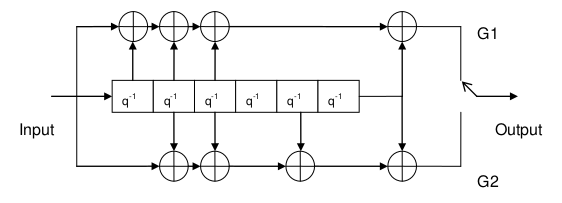
\includegraphics[width=\columnwidth]{figs/FEC.png}
\centering
\captionsetup{justification=centering}
\caption{FEC Encoding}
\label{fig:FEC}
\end{figure}
\newpage
\begin{table}[h]
%\centering
%%%%%%%%%%%%%%%%%%%%%%%%%%%%%%%%%%%%%%%%%%%%%%%%%%%%%%%%%%%%%%%%%%%%%%
%%                                                                  %%
%%  This is the header of a LaTeX2e file exported from Gnumeric.    %%
%%                                                                  %%
%%  This file can be compiled as it stands or included in another   %%
%%  LaTeX document. The table is based on the longtable package so  %%
%%  the longtable options (headers, footers...) can be set in the   %%
%%  preamble section below (see PRAMBLE).                           %%
%%                                                                  %%
%%  To include the file in another, the following two lines must be %%
%%  in the including file:                                          %%
%%        \def\inputGnumericTable{}                                 %%
%%  at the beginning of the file and:                               %%
%%        \input{name-of-this-file.tex}                             %%
%%  where the table is to be placed. Note also that the including   %%
%%  file must use the following packages for the table to be        %%
%%  rendered correctly:                                             %%
%%    \usepackage[latin1]{inputenc}                                 %%
%%    \usepackage{color}                                            %%
%%    \usepackage{array}                                            %%
%%    \usepackage{longtable}                                        %%
%%    \usepackage{calc}                                             %%
%%    \usepackage{multirow}                                         %%
%%    \usepackage{hhline}                                           %%
%%    \usepackage{ifthen}                                           %%
%%  optionally (for landscape tables embedded in another document): %%
%%    \usepackage{lscape}                                           %%
%%                                                                  %%
%%%%%%%%%%%%%%%%%%%%%%%%%%%%%%%%%%%%%%%%%%%%%%%%%%%%%%%%%%%%%%%%%%%%%%



%%  This section checks if we are begin input into another file or  %%
%%  the file will be compiled alone. First use a macro taken from   %%
%%  the TeXbook ex 7.7 (suggestion of Han-Wen Nienhuys).            %%
\def\ifundefined#1{\expandafter\ifx\csname#1\endcsname\relax}


%%  Check for the \def token for inputed files. If it is not        %%
%%  defined, the file will be processed as a standalone and the     %%
%%  preamble will be used.                                          %%
\ifundefined{inputGnumericTable}

%%  We must be able to close or not the document at the end.        %%
	\def\gnumericTableEnd{\end{document}}


%%%%%%%%%%%%%%%%%%%%%%%%%%%%%%%%%%%%%%%%%%%%%%%%%%%%%%%%%%%%%%%%%%%%%%
%%                                                                  %%
%%  This is the PREAMBLE. Change these values to get the right      %%
%%  paper size and other niceties.                                  %%
%%                                                                  %%
%%%%%%%%%%%%%%%%%%%%%%%%%%%%%%%%%%%%%%%%%%%%%%%%%%%%%%%%%%%%%%%%%%%%%%

	\documentclass[12pt%
			  %,landscape%
                    ]{report}
       \usepackage[latin1]{inputenc}
       \usepackage{fullpage}
       \usepackage{color}
       \usepackage{array}
       \usepackage{longtable}
       \usepackage{calc}
       \usepackage{multirow}
       \usepackage{hhline}
       \usepackage{ifthen}

	\begin{document}


%%  End of the preamble for the standalone. The next section is for %%
%%  documents which are included into other LaTeX2e files.          %%
\else

%%  We are not a stand alone document. For a regular table, we will %%
%%  have no preamble and only define the closing to mean nothing.   %%
    \def\gnumericTableEnd{}

%%  If we want landscape mode in an embedded document, comment out  %%
%%  the line above and uncomment the two below. The table will      %%
%%  begin on a new page and run in landscape mode.                  %%
%       \def\gnumericTableEnd{\end{landscape}}
%       \begin{landscape}


%%  End of the else clause for this file being \input.              %%
\fi

%%%%%%%%%%%%%%%%%%%%%%%%%%%%%%%%%%%%%%%%%%%%%%%%%%%%%%%%%%%%%%%%%%%%%%
%%                                                                  %%
%%  The rest is the gnumeric table, except for the closing          %%
%%  statement. Changes below will alter the table's appearance.     %%
%%                                                                  %%
%%%%%%%%%%%%%%%%%%%%%%%%%%%%%%%%%%%%%%%%%%%%%%%%%%%%%%%%%%%%%%%%%%%%%%

\providecommand{\gnumericmathit}[1]{#1} 
%%  Uncomment the next line if you would like your numbers to be in %%
%%  italics if they are italizised in the gnumeric table.           %%
%\renewcommand{\gnumericmathit}[1]{\mathit{#1}}
\providecommand{\gnumericPB}[1]%
{\let\gnumericTemp=\\#1\let\\=\gnumericTemp\hspace{0pt}}
 \ifundefined{gnumericTableWidthDefined}
        \newlength{\gnumericTableWidth}
        \newlength{\gnumericTableWidthComplete}
        \newlength{\gnumericMultiRowLength}
        \global\def\gnumericTableWidthDefined{}
 \fi
%% The following setting protects this code from babel shorthands.  %%
 \ifthenelse{\isundefined{\languageshorthands}}{}{\languageshorthands{english}}
%%  The default table format retains the relative column widths of  %%
%%  gnumeric. They can easily be changed to c, r or l. In that case %%
%%  you may want to comment out the next line and uncomment the one %%
%%  thereafter                                                      %%
\providecommand\gnumbox{\makebox[0pt]}
%%\providecommand\gnumbox[1][]{\makebox}

%% to adjust positions in multirow situations                       %%
\setlength{\bigstrutjot}{\jot}
\setlength{\extrarowheight}{\doublerulesep}

%%  The \setlongtables command keeps column widths the same across  %%
%%  pages. Simply comment out next line for varying column widths.  %%
\setlongtables

\setlength\gnumericTableWidth{%
	30pt+%
	30pt+%
0pt}
\def\gumericNumCols{2}
\setlength\gnumericTableWidthComplete{\gnumericTableWidth+%
         \tabcolsep*\gumericNumCols*2+\arrayrulewidth*\gumericNumCols}
\ifthenelse{\lengthtest{\gnumericTableWidthComplete > \linewidth}}%
         {\def\gnumericScale{\ratio{\linewidth-%
                        \tabcolsep*\gumericNumCols*2-%
                        \arrayrulewidth*\gumericNumCols}%
{\gnumericTableWidth}}}%
{\def\gnumericScale{1}}

%%%%%%%%%%%%%%%%%%%%%%%%%%%%%%%%%%%%%%%%%%%%%%%%%%%%%%%%%%%%%%%%%%%%%%
%%                                                                  %%
%% The following are the widths of the various columns. We are      %%
%% defining them here because then they are easier to change.       %%
%% Depending on the cell formats we may use them more than once.    %%
%%                                                                  %%
%%%%%%%%%%%%%%%%%%%%%%%%%%%%%%%%%%%%%%%%%%%%%%%%%%%%%%%%%%%%%%%%%%%%%%

\ifthenelse{\isundefined{\gnumericColA}}{\newlength{\gnumericColA}}{}\settowidth{\gnumericColA}{\begin{tabular}{@{}p{115pt*\gnumericScale}@{}}x\end{tabular}}
\ifthenelse{\isundefined{\gnumericColB}}{\newlength{\gnumericColB}}{}\settowidth{\gnumericColB}{\begin{tabular}{@{}p{115pt*\gnumericScale}@{}}x\end{tabular}}

\begin{longtable}[c]{%
	b{\gnumericColA}%
	b{\gnumericColB}%
	}

%%%%%%%%%%%%%%%%%%%%%%%%%%%%%%%%%%%%%%%%%%%%%%%%%%%%%%%%%%%%%%%%%%%%%%
%%  The longtable options. (Caption, headers... see Goosens, p.124) %%
%	\caption{The Table Caption.}             \\	%
% \hline	% Across the top of the table.
%%  The rest of these options are table rows which are placed on    %%
%%  the first, last or every page. Use \multicolumn if you want.    %%

%%  Header for the first page.                                      %%
%	\multicolumn{2}{c}{The First Header} \\ \hline 
%	\multicolumn{1}{c}{colTag}	%Column 1
%	&\multicolumn{1}{c}{colTag}	\\ \hline %Last column
%	\endfirsthead

%%  The running header definition.                                  %%
%	\hline
%	\multicolumn{2}{l}{\ldots\small\slshape continued} \\ \hline
%	\multicolumn{1}{c}{colTag}	%Column 1
%	&\multicolumn{1}{c}{colTag}	\\ \hline %Last column
%	\endhead

%%  The running footer definition.                                  %%
%	\hline
%	\multicolumn{2}{r}{\small\slshape continued\ldots} \\
%	\endfoot

%%  The ending footer definition.                                   %%
%	\multicolumn{2}{c}{That's all folks} \\ \hline 
%	\endlastfoot
%%%%%%%%%%%%%%%%%%%%%%%%%%%%%%%%%%%%%%%%%%%%%%%%%%%%%%%%%%%%%%%%%%%%%%

\hhline{|-|-|}
	 \multicolumn{1}{|p{\gnumericColA}|}%
	{\gnumericPB{\raggedright}\gnumbox[l]{\textbf{Parameter}}}
	&\multicolumn{1}{p{\gnumericColB}|}%
	{\gnumericPB{\raggedright}\gnumbox[l]{\hspace{1.2cm}\textbf{Value}}}
\\

\hhline{|--|}
	 \multicolumn{1}{|p{\gnumericColA}|}%
	{\gnumericPB{\raggedright}\gnumbox[l]{Coding Rate}}
	&\multicolumn{1}{p{\gnumericColB}|}%
	{\gnumericPB{\raggedright}\gnumbox[l]{\hspace{1.6cm}$\frac{1}{2}$}}
\\
\hhline{|--|}
	 \multicolumn{1}{|p{\gnumericColA}|}%
	{\gnumericPB{\raggedright}\gnumbox[l]{Coding Scheme}}
	&\multicolumn{1}{p{\gnumericColB}|}%
	{\gnumericPB{\raggedright}\gnumbox[l]{\hspace{0.8cm}Convolution}}
\\
\hhline{|--|}
	 \multicolumn{1}{|p{\gnumericColA}|}%
	{\gnumericPB{\raggedright}\gnumbox[l]{Constraint Length}}
	&\multicolumn{1}{p{\gnumericColB}|}%
	{\gnumericPB{\raggedright}\gnumbox[l]{\hspace{1.6cm}$7$}}
\\
\hhline{|--|}
	 \multicolumn{1}{|p{\gnumericColA}|}%
	{\gnumericPB{\raggedright}\gnumbox[l]{Generator Polynomial}}
	&\multicolumn{1}{p{\gnumericColB}|}%
	{\gnumericPB{\raggedright}\gnumbox[l]{\hspace{1cm}G1=(171)o}}
\\
\hhline{|  |}
	 \multicolumn{1}{|p{\gnumericColA}|}%
	{\gnumericPB{\raggedright}\gnumbox[l]{}}
	&\multicolumn{1}{p{\gnumericColB}|}%
	{\gnumericPB{\raggedright}\gnumbox[l]{\hspace{1cm}G2=(133)o}}
\\
\hhline{|--|}
	 \multicolumn{1}{|p{\gnumericColA}|}%
	{\gnumericPB{\raggedright}\gnumbox[l]{Encoding Sequence}}
	&\multicolumn{1}{p{\gnumericColB}|}%
	{\gnumericPB{\raggedright}\gnumbox[l]{\hspace{1cm}G$1$ then G$2$}}
\\
\hhline{|--|}
\end{longtable}

\ifthenelse{\isundefined{\languageshorthands}}{}{\languageshorthands{\languagename}}
\gnumericTableEnd

\vspace{3mm}
\caption{FEC encoding parameters}
\label{table:fec_enc}
\end{table}
\subsection{Interleaving}
Interleaving is a technique used in digital communication systems to improve the resilience of transmitted data against burst errors, which are clusters of errors occurring close together in time. This technique involves rearranging the order of transmitted data, spreading errors over time, and enabling more effective error correction by error detection and correction codes. Interleaving is commonly used in various communication systems, including satellite communication, wireless communication, and storage systems.
\subsubsection{Burst Errors:}
\begin{enumerate}
    \item Burst errors are consecutive errors that occur within a short time frame. 
    \item These errors can result from various factors such as atmospheric conditions, interference, or other channel impairments.
\end{enumerate}
\subsubsection{Motivation for Interleaving:}
\begin{enumerate}
    \item Interleaving is motivated by the need to mitigate the impact of burst errors.
    \item By rearranging the order of transmitted data, interleaving helps disperse errors, preventing them from affecting consecutive bits or symbols.
\end{enumerate}
\subsubsection{Interleaving Process:}
\begin{enumerate}
    \item Interleaving is typically performed in blocks or frames of data.
    \item The data within each block is rearranged systematically, changing the order of symbols or bits.
\end{enumerate}
\subsubsection{Benefits of Interleaving:}
\begin{enumerate}
    \item Improved Error Correction: Interleaving allows error correction codes to more effectively correct errors because they are spread out over time.
    \item Increased Robustness: Interleaving enhances the system's ability to recover from burst errors, providing a more reliable communication link.
\end{enumerate}
The $584$ symbols of FEC encoded navigation data  is interleaved using a block interleaver with n columns and k rows. Data is written in columns and then, read in rows.
\\
Any burst errors during the data transmission can be corrected by interleaving. In matrix interleaving, input symbols are filled into a matrix column wise and read at the output row wise. This will spread the burst error, if any, during the transmission. For SPS, data is filled into matrix of size $73$ by $8$($73$ columns, $8$ rows).
\subsection{Sync word and Tail bits}
Each subframe has a $16$ bit word synchronization pattern which is not encoded. Sync pattern is $EB90$ Hex. Tail bits consist of $6$ zero value bits added to the subframe and tail bits are part of FEC encoding. 

Any burst errors during the data transmission can be corrected by interleaving. In matrix interleaving, input symbols are filled into a matrix column wise and read at the output row wise. This will spread the burst error, if any, during the transmission. For SPS, data is filled into matrix of size $73$ by $8$($73$ columns, $8$ rows).
\subsection{Sync word and Tail bits}
Each subframe has a $16$ bit word synchronization pattern which is not encoded. Sync pattern is $EB90$ Hex. Tail bits consist of $6$ zero value bits added to the subframe and tail bits are part of FEC encoding. 

\subsection{Cyclic Redundancy Check(CRC)}
The parity coding of data signal follows $24$Q polynomial for each subframe. $24$ bits of CRC parity will provide protection against burst as well as random errors with undetected error probability of $2^{-24}$ for all channel bit error probabilities $0.5$.

\begin{equation}
    g(X) = \sum_{i = 0}^{24}g_{i}X^i\;\; 
\end{equation}

    $g_{i}=1$; for $i = 0,1,3,4,5,6,7,10,11,14,17,18,23,24$ \\
          = 0 otherwise
\\
\textbf{Transmitter End}:
\\ 1. Add k-1 zeroes at the end of the data, k being the lenght of crc polynomial.
\\2. Using modulo-2 binary division, divide data with polynomial, store remainder.
\\3. Append remainder at the end of the data, forming encoded data.
\\\textbf{Receiver End}:
\\1. Perform modulo-2 division on received data and polynomial. If the remainder is 0, no error has occured.Else, atleast one error has occured.
\section{Modulation}

\subsection{Standard Positioning Service}
The SPS signal is BPSK(1) modulated on L5 and S bands. The navigation data at data rate of $50$ sps (1/2 rate FEC encoded) is modulo $2$ added to PRN code chipped at $1.023$ Mcps. The CDMA modulated code is upconverted by the L5 and S carriers at $1176.45$ MHz and $2492.028$ MHz respectively. However, this simulation does not carry out this upconversion.

\subsection{Baseband Modulation}
The carrier signal is modulated by BPSK(1), Data channel BOC(5,2), and Pilot Channel BOC(5,2). To have a constant envelop when passed through power amplifier, we add additional signal called interplex signal.
The basic concept of BPSK(n) (Binary Phase Shift Keying)implemented in very basic by multiplying the local oscillator by 1 or -1 for a 1 or 0 chip respectively. here,the "(n)" notation means that the signal has a chip rate of n*$f_0$ ,where $f_0$ is 1.023 Mcps(Mega chips per second).

Binary offset carrier (BOC) modulation allows interoperability of satellite navigation systems. It is currently used in the US GPS system, Indian IRNSS system and in Galileo and is a square sub-carrier modulation, where a signal is multiplied by a rectangular sub-carrier of frequency $f_{sc}$ equal to or greater than the chip rate. Following this sub-carrier multiplication, the spectrum of the signal is divided into two parts, therefore BOC modulation is also known as a split-spectrum modulation. \\

The main idea behind BOC modulation is to reduce the interference with BPSK-modulated signal, which has a sinc function shaped spectrum. Therefore, BPSK-modulated signals have most of their spectral energy concentrated around the carrier frequency, while BOC-modulated signals have low energy around the carrier frequency and two main spectral lobes further away from the carrier (thus, the name of split-spectrum). 
A BOC waveform is typically denoted via BOC(m, n) or BOC ($f_{sc}$ , $f_c$), where $f_{ sc}$ is the sub-carrier frequency,$f_c$ is the chip frequency, m = $f_{sc}$ / $f_{ref}$ , n = $f_c$ / $f_{ref}$, and $f_{ref}$ = 1.023Mcps is the reference chip frequency of NavIC signal.

\subsubsection{Mathematical Equations}
The following equations describe baseband signals for L5 and S band navigation data.
\\
\textbf{SPS Data Signal:}
\begin{equation}
	s_{sps}(t) = \sum_{i=-\infty}^{\infty} c_{sps}(\abs{i}_{L\_sps}) . d_{sps}(\sbrak{i}_{CD\_sps}) . \rect_{T_{c,sps}}(t-iT_{c,sps})
\end{equation}
\textbf{RS BOC Pilot Signal:}
\begin{equation}
	s_{rs\_p}(t) = \sum_{i=-\infty}^{\infty} c_{rs\_p}(\abs{i}_{L\_rs\_p}) . \rect_{Tc,rs\_p}(t-iT_{c,rs\_p}). sc_{rs\_p}(t,0)
\end{equation}
\textbf{RS BOC Signal:}
%\begin{equation}
\begin{multline}
	s_{rs\_d}(t) = \sum_{i=-\infty}^{\infty} c_{rs\_d}(\abs{i}_{L\_rs\_d}) . d_{rs\_d}(\sbrak{i}_{CD\_rs\_d}).  \\ 
	                       \rect_{T_{c,rs\_d}}(t-iT_{c,rs\_d}). sc_{rs_d}(t,0)
\end{multline}
%\end{equation}
The sub-carrier is defined as:
\begin{equation}
	sc_x(t,\phi) = \sgn\sbrak{sin(2 \pi f_{sc,x}t + \phi)}
\end{equation}

\noindent The IRNSS RS data and pilot BOC signals are sinBOC. Hence the subcarrier phase $\phi=0$.
The complex envelope of composite signal with Interplex signal (I(t)) is:
\begin{equation}
s(t) = \dfrac{1}{3} \sbrak{\sqrt{2} (s_{sps}(t) + s_{rs\_p}(t)) + j(2. s_{rs\_d}(t) - I(t))} 
\end{equation}

\noindent The Interplex signal $I(t)$ is generated to realize the constant envelope composite signal. The operation $\abs{i}_X$ gives the code chip index for any signal. Similarly $[i]_X$ gives data bit index for any signal.
Symbol definitions are given in below table \ref{table:symbdesc}.

\begin{table}[h]
%\centering
%%%%%%%%%%%%%%%%%%%%%%%%%%%%%%%%%%%%%%%%%%%%%%%%%%%%%%%%%%%%%%%%%%%%%%
%%                                                                  %%
%%  This is the header of a LaTeX2e file exported from Gnumeric.    %%
%%                                                                  %%
%%  This file can be compiled as it stands or included in another   %%
%%  LaTeX document. The table is based on the longtable package so  %%
%%  the longtable options (headers, footers...) can be set in the   %%
%%  preamble section below (see PRAMBLE).                           %%
%%                                                                  %%
%%  To include the file in another, the following two lines must be %%
%%  in the including file:                                          %%
%%        \def\inputGnumericTable{}                                 %%
%%  at the beginning of the file and:                               %%
%%        \input{name-of-this-file.tex}                             %%
%%  where the table is to be placed. Note also that the including   %%
%%  file must use the following packages for the table to be        %%
%%  rendered correctly:                                             %%
%%    \usepackage[latin1]{inputenc}                                 %%
%%    \usepackage{color}                                            %%
%%    \usepackage{array}                                            %%
%%    \usepackage{longtable}                                        %%
%    \usepackage{calc}                                             %%
%%    \usepackage{multirow}                                         %%
%%    \usepackage{hhline}                                           %%
%%    \usepackage{ifthen}                                           %%
%%  optionally (for landscape tables embedded in another document): %%
%%    \usepackage{lscape}                                           %%
%%                                                                  %%
%%%%%%%%%%%%%%%%%%%%%%%%%%%%%%%%%%%%%%%%%%%%%%%%%%%%%%%%%%%%%%%%%%%%%%



%%  This section checks if we are begin input into another file or  %%
%%  the file will be compiled alone. First use a macro taken from   %%
%%  the TeXbook ex 7.7 (suggestion of Han-Wen Nienhuys).            %%
\def\ifundefined#1{\expandafter\ifx\csname#1\endcsname\relax}


%%  Check for the \def token for inputed files. If it is not        %%
%%  defined, the file will be processed as a standalone and the     %%
%%  preamble will be used.                                          %%
\ifundefined{inputGnumericTable}

%%  We must be able to close or not the document at the end.        %%
	\def\gnumericTableEnd{\end{document}}


%%%%%%%%%%%%%%%%%%%%%%%%%%%%%%%%%%%%%%%%%%%%%%%%%%%%%%%%%%%%%%%%%%%%%%
%%                                                                  %%
%%  This is the PREAMBLE. Change these values to get the right      %%
%%  paper size and other niceties.                                  %%
%%                                                                  %%
%%%%%%%%%%%%%%%%%%%%%%%%%%%%%%%%%%%%%%%%%%%%%%%%%%%%%%%%%%%%%%%%%%%%%%

	\documentclass[12pt%
			  %,landscape%
                    ]{report}
       \usepackage[latin1]{inputenc}
       \usepackage{fullpage}
       \usepackage{color}
       \usepackage{array}
       \usepackage{longtable}
       \usepackage{calc}
       \usepackage{multirow}
       \usepackage{hhline}
       \usepackage{ifthen}

	\begin{document}


%%  End of the preamble for the standalone. The next section is for %%
%%  documents which are included into other LaTeX2e files.          %%
\else

%%  We are not a stand alone document. For a regular table, we will %%
%%  have no preamble and only define the closing to mean nothing.   %%
    \def\gnumericTableEnd{}

%%  If we want landscape mode in an embedded document, comment out  %%
%%  the line above and uncomment the two below. The table will      %%
%%  begin on a new page and run in landscape mode.                  %%
%       \def\gnumericTableEnd{\end{landscape}}
%       \begin{landscape}


%%  End of the else clause for this file being \input.              %%
\fi

%%%%%%%%%%%%%%%%%%%%%%%%%%%%%%%%%%%%%%%%%%%%%%%%%%%%%%%%%%%%%%%%%%%%%%
%%                                                                  %%
%%  The rest is the gnumeric table, except for the closing          %%
%%  statement. Changes below will alter the table's appearance.     %%
%%                                                                  %%
%%%%%%%%%%%%%%%%%%%%%%%%%%%%%%%%%%%%%%%%%%%%%%%%%%%%%%%%%%%%%%%%%%%%%%

\providecommand{\gnumericmathit}[1]{#1} 
%%  Uncomment the next line if you would like your numbers to be in %%
%%  italics if they are italizised in the gnumeric table.           %%
%\renewcommand{\gnumericmathit}[1]{\mathit{#1}}
\providecommand{\gnumericPB}[1]%
{\let\gnumericTemp=\\#1\let\\=\gnumericTemp\hspace{0pt}}
 \ifundefined{gnumericTableWidthDefined}
        \newlength{\gnumericTableWidth}
        \newlength{\gnumericTableWidthComplete}
        \newlength{\gnumericMultiRowLength}
        \global\def\gnumericTableWidthDefined{}
 \fi
%% The following setting protects this code from babel shorthands.  %%
 \ifthenelse{\isundefined{\languageshorthands}}{}{\languageshorthands{english}}
%%  The default table format retains the relative column widths of  %%
%%  gnumeric. They can easily be changed to c, r or l. In that case %%
%%  you may want to comment out the next line and uncomment the one %%
%%  thereafter                                                      %%
\providecommand\gnumbox{\makebox[0pt]}
%%\providecommand\gnumbox[1][]{\makebox}

%% to adjust positions in multirow situations                       %%
\setlength{\bigstrutjot}{\jot}
\setlength{\extrarowheight}{\doublerulesep}

%%  The \setlongtables command keeps column widths the same across  %%
%%  pages. Simply comment out next line for varying column widths.  %%
\setlongtables

\setlength\gnumericTableWidth{%
	80pt+%
	180pt+%
0pt}
\def\gumericNumCols{2}
\setlength\gnumericTableWidthComplete{\gnumericTableWidth+%
         \tabcolsep*\gumericNumCols*2+\arrayrulewidth*\gumericNumCols}
\ifthenelse{\lengthtest{\gnumericTableWidthComplete > \linewidth}}%
         {\def\gnumericScale{\ratio{\linewidth-%
                        \tabcolsep*\gumericNumCols*2-%
                        \arrayrulewidth*\gumericNumCols}%
{\gnumericTableWidth}}}%
{\def\gnumericScale{1}}

%%%%%%%%%%%%%%%%%%%%%%%%%%%%%%%%%%%%%%%%%%%%%%%%%%%%%%%%%%%%%%%%%%%%%%
%%                                                                  %%
%% The following are the widths of the various columns. We are      %%
%% defining them here because then they are easier to change.       %%
%% Depending on the cell formats we may use them more than once.    %%
%%                                                                  %%
%%%%%%%%%%%%%%%%%%%%%%%%%%%%%%%%%%%%%%%%%%%%%%%%%%%%%%%%%%%%%%%%%%%%%%

\ifthenelse{\isundefined{\gnumericColA}}{\newlength{\gnumericColA}}{}\settowidth{\gnumericColA}{\begin{tabular}{@{}p{80pt*\gnumericScale}@{}}x\end{tabular}}
\ifthenelse{\isundefined{\gnumericColB}}{\newlength{\gnumericColB}}{}\settowidth{\gnumericColB}{\begin{tabular}{@{}p{180pt*\gnumericScale}@{}}x\end{tabular}}

\begin{longtable}[c]{%
	b{\gnumericColA}%
	b{\gnumericColB}%
	}

%%%%%%%%%%%%%%%%%%%%%%%%%%%%%%%%%%%%%%%%%%%%%%%%%%%%%%%%%%%%%%%%%%%%%%
%%  The longtable options. (Caption, headers... see Goosens, p.124) %%
%	\caption{The Table Caption.}             \\	%
% \hline	% Across the top of the table.
%%  The rest of these options are table rows which are placed on    %%
%%  the first, last or every page. Use \multicolumn if you want.    %%

%%  Header for the first page.                                      %%
%	\multicolumn{2}{c}{The First Header} \\ \hline 
%	\multicolumn{1}{c}{colTag}	%Column 1
%	&\multicolumn{1}{c}{colTag}	\\ \hline %Last column
%	\endfirsthead

%%  The running header definition.                                  %%
%	\hline
%	\multicolumn{2}{l}{\ldots\small\slshape continued} \\ \hline
%	\multicolumn{1}{c}{colTag}	%Column 1
%	&\multicolumn{1}{c}{colTag}	\\ \hline %Last column
%	\endhead

%%  The running footer definition.                                  %%
%	\hline
%	\multicolumn{2}{r}{\small\slshape continued\ldots} \\
%	\endfoot

%%  The ending footer definition.                                   %%
%	\multicolumn{2}{c}{That's all folks} \\ \hline 
%	\endlastfoot
%%%%%%%%%%%%%%%%%%%%%%%%%%%%%%%%%%%%%%%%%%%%%%%%%%%%%%%%%%%%%%%%%%%%%%

\hhline{|-|-}
	 \multicolumn{1}{|p{\gnumericColA}|}%
	{\gnumericPB{\raggedright}\gnumbox[l]{\hspace*{1cm}\textbf{Symbol}}}
	&\multicolumn{1}{p{\gnumericColB}|}%
	{\gnumericPB{\raggedright}\gnumbox[l]{\hspace*{2cm}\textbf{Definition}}}
\\
\hhline{|--|}
	 \multicolumn{1}{|p{\gnumericColA}|}%
	{\gnumericPB{\raggedright}\gnumbox[l]{\hspace{1cm}A}}
	&\multicolumn{1}{p{\gnumericColB}|}%
	{\gnumericPB{\raggedright}\gnumbox[l]{ received signal amplitude}}
\\
\hhline{|--|}
	 \multicolumn{1}{|p{\gnumericColA}|}%
	{\gnumericPB{\raggedright}\gnumbox[l]{\hspace{1cm}$f_c$}}
	&\multicolumn{1}{p{\gnumericColB}|}%
	{\gnumericPB{\raggedright}\gnumbox[l]{carrier frequency}}
\\
\hhline{|--|}
	 \multicolumn{1}{|p{\gnumericColA}|}%
	{\gnumericPB{\raggedright}\gnumbox[l]{\hspace{1cm}$f_{sub}$}}
	&\multicolumn{1}{p{\gnumericColB}|}%
	{\gnumericPB{\raggedright}\gnumbox[l]{subcarrier frequency}}
\\
\hhline{|--|}
	 \multicolumn{1}{|p{\gnumericColA}|}%
	{\gnumericPB{\raggedright}\gnumbox[l]{\hspace{1cm}t}}
	&\multicolumn{1}{p{\gnumericColB}|}%
	{\gnumericPB{\raggedright}\gnumbox[l]{time}}
\\
\hhline{|--|}
	 \multicolumn{1}{|p{\gnumericColA}|}%
	{\gnumericPB{\raggedright}\gnumbox[l]{\hspace{1cm}q}}
	&\multicolumn{1}{p{\gnumericColB}|}%
	{\gnumericPB{\raggedright}\gnumbox[l]{ phase offset}}
\\
\hhline{|--|}
	 \multicolumn{1}{|p{\gnumericColA}|}%
	{\gnumericPB{\raggedright}\gnumbox[l]{\hspace{1cm}s(t)}}
	&\multicolumn{1}{p{\gnumericColB}|}%
	{\gnumericPB{\raggedright}\gnumbox[l]{BPSK signal transmitted data(-1,1)}}
\\
\hhline{|-|-|}
\end{longtable}

\ifthenelse{\isundefined{\languageshorthands}}{}{\languageshorthands{\languagename}}
\gnumericTableEnd

\vspace{3mm}
\caption{Symbol Description}
\label{table:symbdesc}
\end{table}

The functions for data generation, SPS-PRN sequence generation and baseband modulation are present in the below code.
\begin{lstlisting}
    codes/transmitter/transmitter.py
\end{lstlisting}
\let\cleardoublepage\clearpage
